\chapter{Quality Assurance}
\label{vl:tc-QA}

\section{Overview of DUNE Quality Assurance}

\dshort{dune} \dword{tc} monitors technical contributions from
collaborating institutions and provides centralized project
coordination functions. One part of this project coordination is
standardizing \dfirst{qa}/\dfirst{qc} practices, one facet
of which is to assist consortia in defining and implementing
\dword{qa}/\dword{qc} plans that maintain uniform, high
standards across the entire detector construction
effort. Figure~\ref{fig:fnal_qa} shows how \dword{dune} \dword{tc}
derives its \dword{qa} program from the principles of the \fnal \dword{qa} program:
requirements are flowed down through the \dword{lbnf-dune}
\dword{qa} program into the \dword{qc} plans developed for consortium fabrication of
detector components and integration and installation of the detector.
\begin{dunefigure}[\fnal QA]{fig:fnal_qa}
  {Flow-down of \fnal \dword{qa} to consortia}
  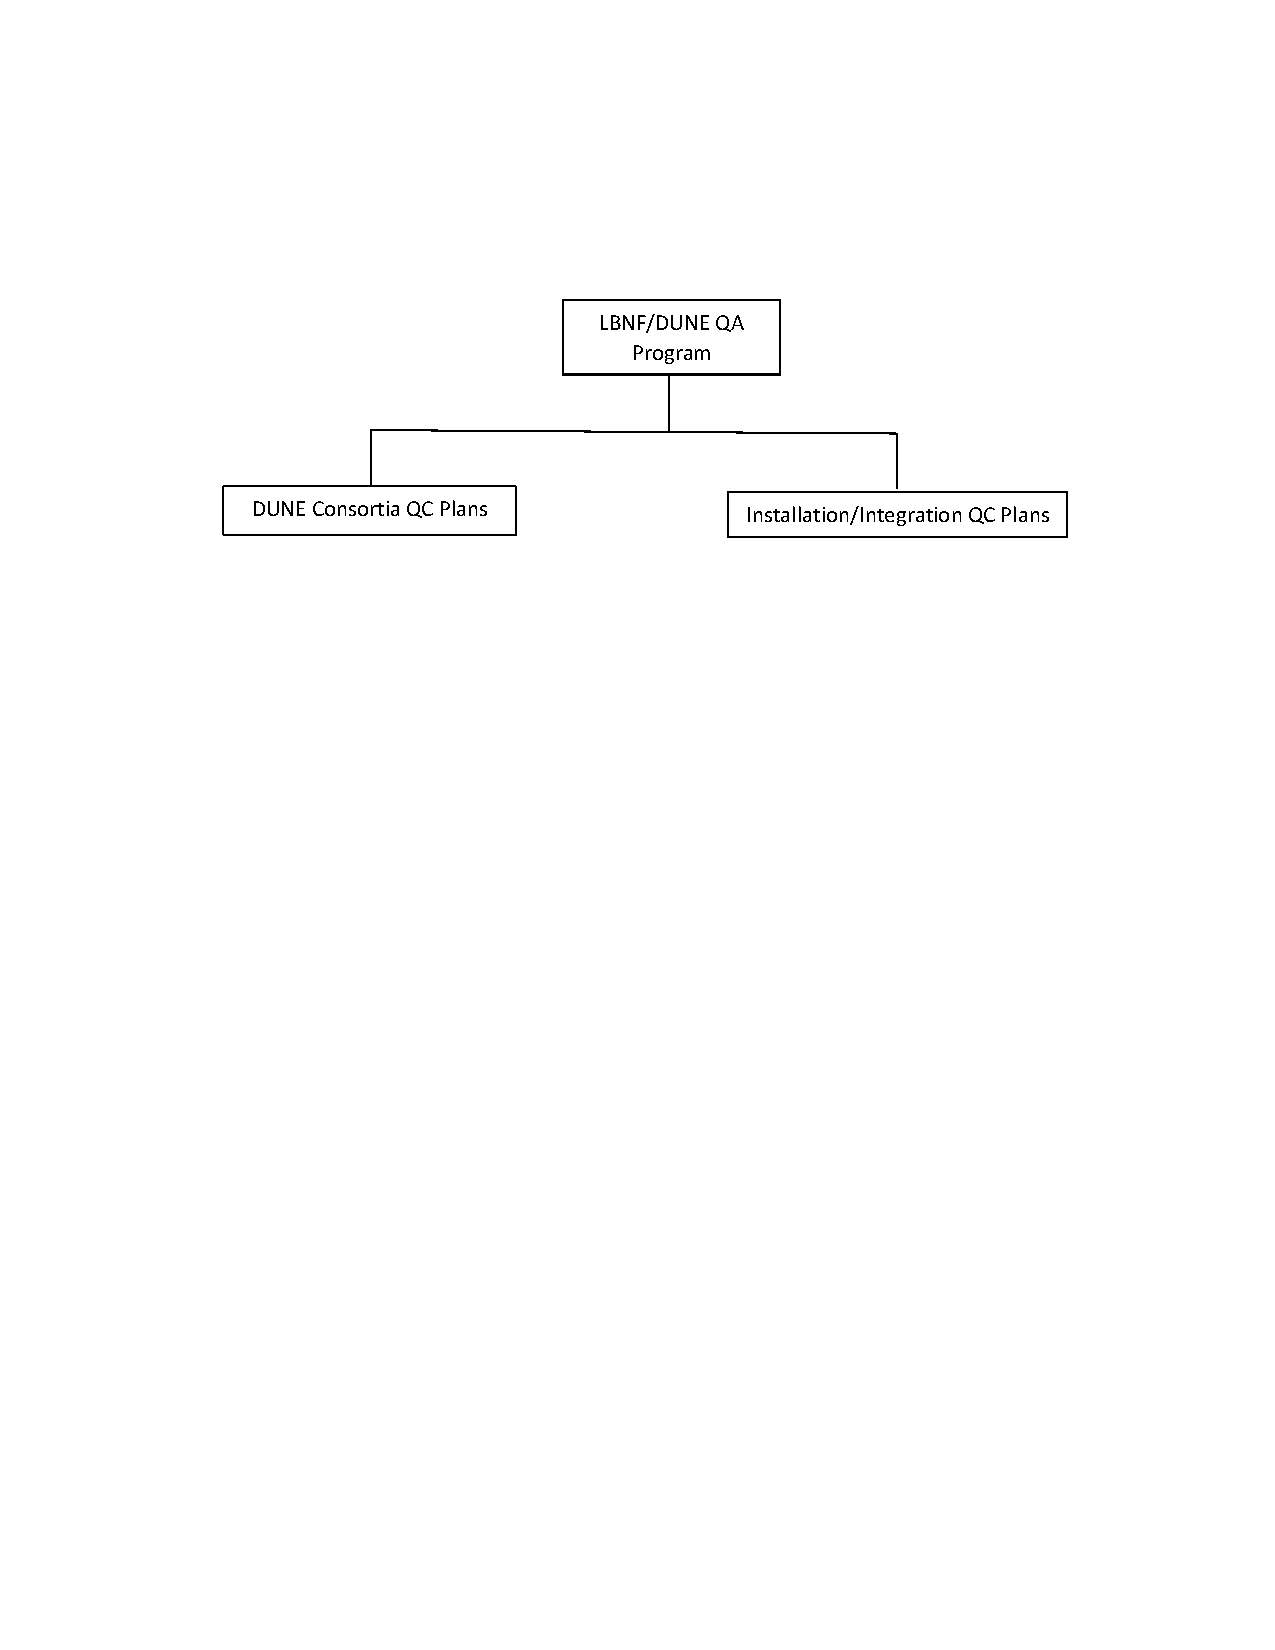
\includegraphics[width=0.85\textwidth]{fnal_qa.pdf}
\end{dunefigure}
The \dword{qa} effort includes design, production readiness, and
progress reviews as appropriate for the \dword{dune} detector
subsystems, as was done for \dword{pdsp} under \dword{tc}
oversight. Installation and operations reviews fall under \dword{jpo}
oversight as is discussed in Chapter~\ref{vl:tc-review}.

\subsection{Purpose}

The primary objective of the \dword{lbnf-dune} \dword{qa} program is
to assure quality in the construction of the \dword{lbnf} facility and
\dword{dune} experiment while providing protection of
\dword{lbnf-dune} personnel, the public and the environment. The
\dword{qa} plan aligns \dword{lbnf-dune} \dword{qa} activities, which
are spread around the world, with the principles of the \fnal Quality
Assurance Manual. The manual identifies the \fnal Integrated Quality
Assurance Program features that serve as the basis for the
\dword{lbnf-dune} \dword{qa} plan.

The \dword{lbnf-dune} \dword{qa} plan outlines the \dword{qa}
requirements for all \dword{lbnf-dune} collaborators and
subcontractors and describes how the requirements will be met.
\Dword{qa} criteria can be satisfied using a graded approach. This
\dword{qa} plan is implemented by the development of quality plans,
procedures, and guides by the consortia to accommodate those specific
quality requirements.

\subsection{Scope}

The \dword{lbnf-dune} \dword{qa} plan provides \Dword{qa}
requirements applicable to all consortia, encompassing all activities
performed from research and development (R\&D) through fabrication and
component commissioning, building on the success of
ProtoDUNE. Consortia are responsible for providing their deliverables,
whether subsystems, components, or services in accordance with
applicable agreements. All parties are responsible for
implementing a quality plan that meet the requirements of the
\dword{lbnf-dune} \dword{qa} plan. Oversight of the work of
the consortia will be the responsibility of the \dword{dune}
\dword{tcoord} and \dword{lbnf-dune} \dword{qa}
manager.

\subsection{Graded Approach}

A key element of the \dword{lbnf-dune} \dword{qa} plan is the
concept of graded approach; that is, applying a level of analysis,
controls, and documentation commensurate with the potential for an
environmental, safety, health, or quality impact. The graded approach
seeks to tailor the kinds and extent of quality controls applied in
the process of fulfilling requirements. Application of the graded
approach entails
\begin{itemize}
  \item identifying activities that present significant \dword{esh}
    and/or quality risk,
  \item defining the activity,
  \item evaluating risk and control choice, and 
  \item documenting and approving the application of the graded
    approach.
\end{itemize}

\section{Quality Assurance Program}

The \dword{lbnf-dune} Systems Engineering teams maintain a
\dword{lbnf-dune} \dword{cmp}, which identifies the \dword{lbnf} project
Configuration Items Data List (CIDL) and Interface Control matrices
that provide the tier structure for the flow down of \dword{qa} plans,
with the \dword{lbnf-dune} \dword{qa} plan as the top tier.

With the
assistance of the \dword{lbnf-dune} \dword{qa} manager, the consortia will develop specific \dword{qa} plans  for
component or system \dword{qa}. Due to the limited scope of
work of some consortia, they may elect to work under the
\dword{lbnf-dune} \dword{qa} plan for their scope of work. In
case of conflict between sets of \dword{qa} requirements, \dword{dune}
\dword{tc} will provide resolution.

With many institutions carrying responsibility for various aspects of
the project, institutional \dword{qa} plans will be reviewed by
\dword{dune} \dword{tc} to ensure compliance with the
\dword{lbnf-dune} \dword{qa} plan. Using a graded approach,
supplements to institutions existing plans will be implemented for
their \dword{dune} scope of work, if necessary.

Overall \dword{qa} supervision, including all activities described
above, is the responsibility of the \dword{dune} \dword{tcoord}.

\subsection{Responsibility for Project Management}

The \dword{dune} consortium leaders manage their projects and are
responsible for achieving performance goals. The
\dword{lbnf-dune} \dword{qa} manager is responsible for
ensuring that a quality system is established, implemented, and
maintained in accordance with requirements. The
\dword{lbnf-dune} \dword{qa} manager reports to the
\dword{dune} \dword{tcoord} and provides oversight and support to
consortium leaders to ensure a consistent quality program.

\dword{dune} consortium leaders are responsible for quality within
their project and report \dword{qa} issues to the \dword{dune}
\dword{tcoord} and \dword{lbnf-dune} \dword{qa}
manager. \dword{dune} consortium leaders designate \dword{qa}
representatives within their organization and delegate, as appropriate, 
work defined in the \dword{lbnf-dune} \dword{qa} plan, as
shown in Fig.~\ref{fig:dune_qa}.
\begin{dunefigure}[DUNE QA organization]{fig:dune_qa}
  {\dword{dune} \dword{qa} organization.}
  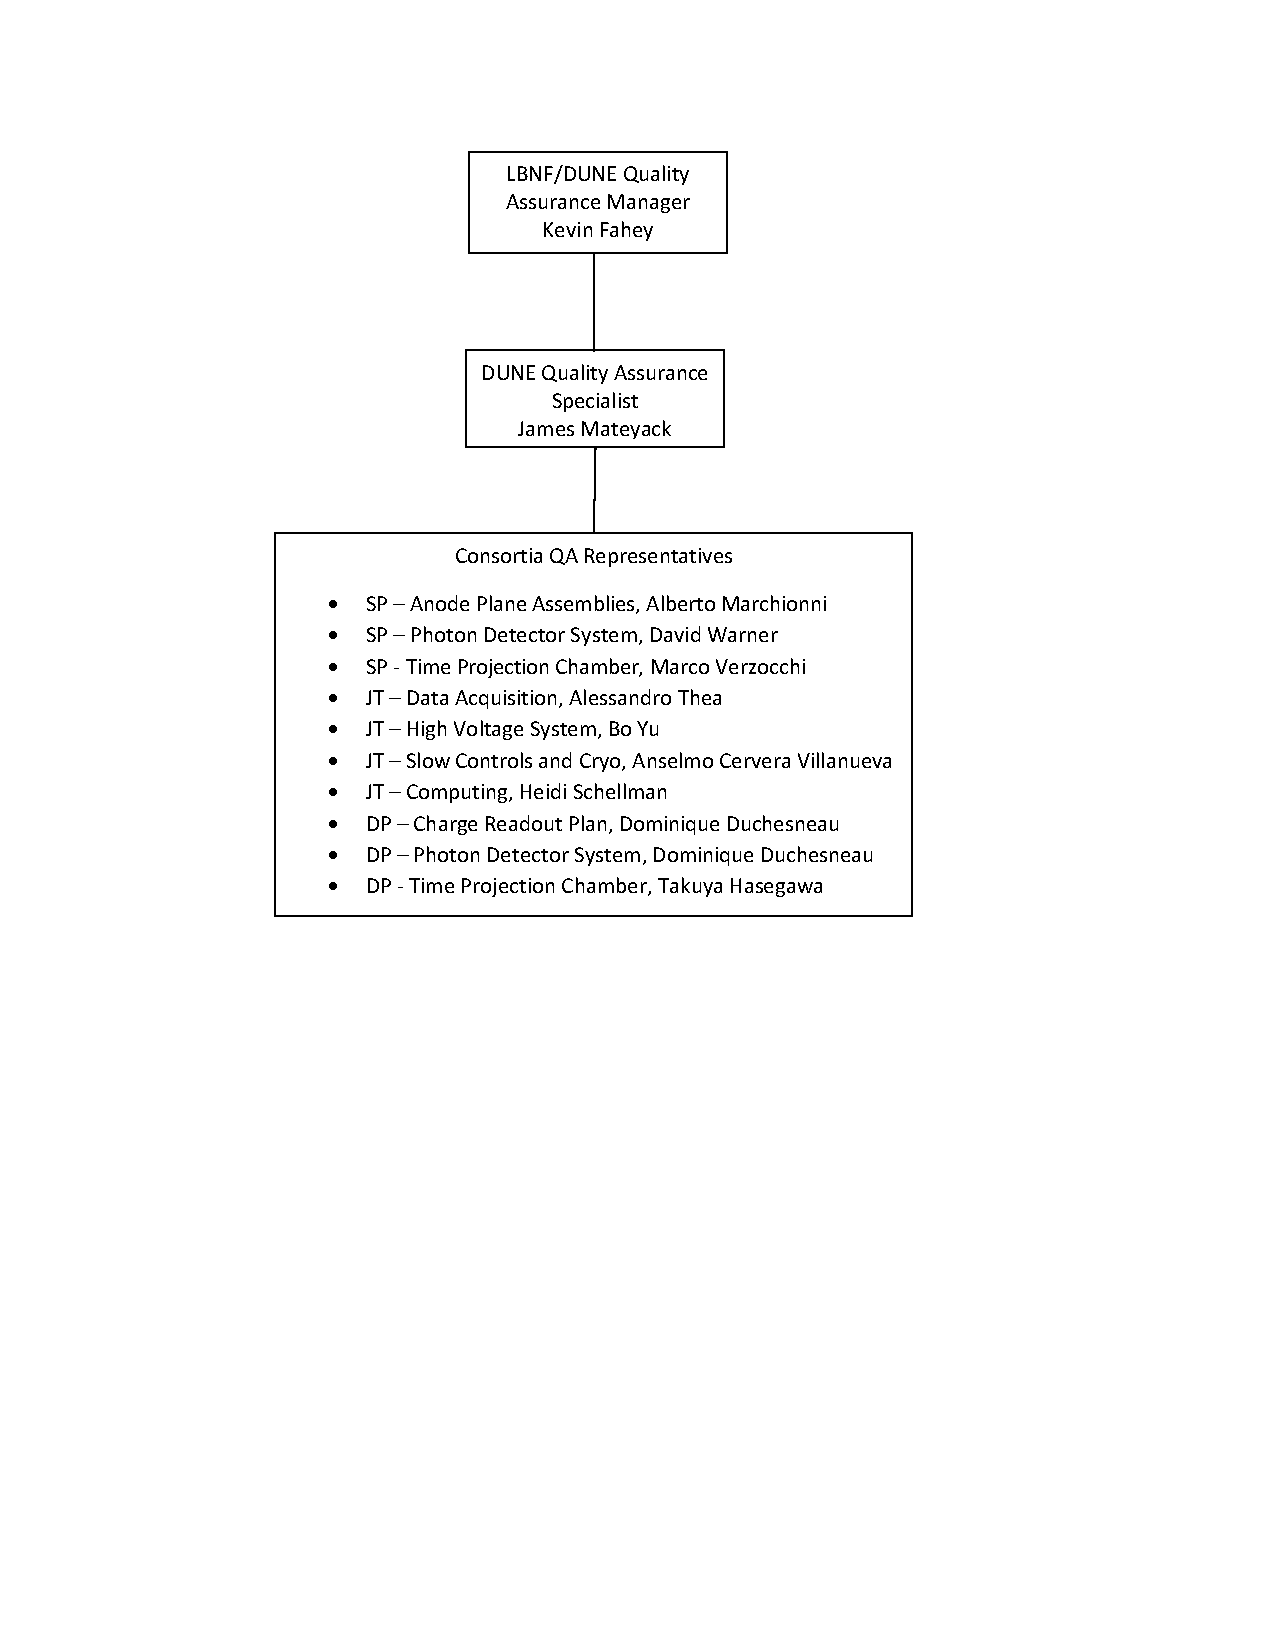
\includegraphics[width=0.75\textwidth]{dune_qa3}
\end{dunefigure}
The \dword{dune} consortium leaders retain overall responsibility for
\dword{qa} even though they have designated a \dword{qa}
representative.

\subsection{Levels of Authority and Interface}

The \dword{dune} Management Plan, the \dword{lbnf-dune} PMP
and the \dword{lbnf-dune} \dword{qa} plan define the
responsibility, authority and interrelation of personnel who manage,
perform, and verify work that affects quality. The \dword{qa} plan
defines the \dword{qa} roles and responsibilities of the \dword{dune}
project.

All consortium members are responsible for the quality of the work that
they do and for using guidance and assistance that is available. Each
has the authority to stop work and report adverse conditions that
affect quality of \dword{dune} products to their respective
\dword{dune} consortium leader and the \dword{lbnf-dune}
\dword{qa} manager. The consortium leader responsible for \dword{dune}
components or systems is required to determine and document their
acceptance criteria. \dword{dune} personnel at each level are
responsible for evaluation of quality through self-assessments;
however, independent quality assessments may also be requested by
project management.  The \dword{lbnf-dune} \dword{qa} manager is
responsible for development, implementation, assessment, and
improvement of the \dword{qa} program.

The \dword{lbnf-dune} \dword{qa} manager is responsible for
periodically reporting on the performance of the quality system to the
\dword{dune} \dword{tcoord} for review and as a basis for improving
the quality system. The \dword{dune} \dword{tcoord} may call for
\dword{qa} plan readiness assessments as the project nears major
milestones. The \dword{dune} \dword{tcoord}, consortium leaders, and
\dword{lbnf-dune} \dword{qa} manager are all responsible for
providing the resources needed to conduct the project successfully,
including those required to manage, perform, and verify work that
affects quality.

\subsection{Quality Assurance Organization}

\dword{lbnf-dune} \dword{qa} manager may request personnel
from the \dword{dune} project to act on behalf of the
\dword{lbnf-dune} \dword{qa} manager to perform quality
assurance functions, based on need, in accordance with the graded
approach described above. The requested personnel must possess
qualifications or receive the appropriate training required to perform
these functions.

The \dword{dune} \dword{qa} Specialist will be responsible for the
following activities:
\begin{itemize}
	\item Cooperatively develop, monitor, and control \dword{dune}
          \dword{qa} procedures to assure compliance with \dword{dune}
          standards and applicable laws;
     \item Provide assistance for \dword{qa}/\dword{qc} matters in project
       plans, including strategizing technical solutions and
       alternatives on \dword{qa}/\dword{qc} matters and assist in developing
       testing plans with project team members;
	   \item Participate in audits, site inspections, accident
             investigations, and monitor trend analysis to identify
             areas of concern and implement improvements;
	\item Interact with all stakeholders on \dword{qa} issues;
      \item Provide guidance and interpretation on routine and complex
        \dword{qa} matters and problems; and
	\item Participate in reviews at collaborating institutions.
\end{itemize}

Each consortium selects a \dword{qa} representative. %for the consortium.  
Each consortium \dword{qa} representative is responsible for
overall coordination of quality requirements to assure they meet
consortium objectives.  The \dword{qa} representative is expected to %responsibilities include
\begin{itemize}
  \item oversee the consortium fabrication facilities for quality
    performance;
  \item interface with the \dword{dune} \dword{qa} specialist on
    consortia \dword{qa} related matters;
  \item monitor the status of all required testing based on the
    consortium \dword{qc} plan;
  \item make sufficient fabrication facility visits to determine
    adequacy of \dword{qc} system performance: check certifications
    of materials and equipment delivered to the facility, spot check
    workmanship, observe testing procedures; and
  \item make or arrange \dwords{ppr} during the fabrication cycle in
    coordination with \dword{tc} and the \dword{jpo} Review Office.
\end{itemize}

Figure~\ref{fig:dune_qa} shows the interface between the
\dword{lbnf-dune} \dword{qa} organization and the consortium \dword{qa}
representatives.  These interfaces will remain when the equipment is
shipped to the far site for installation, but the names may change for
the consortium \dword{qa} representatives.  The consortium \dword{qa}
representatives remain responsible for \dword{qa}/\dword{qc} during the
detector installation process.


\section{Personnel Training and Qualification}

The \dword{dune} consortium leaders are responsible for identifying the
resources to ensure that their team members are adequately trained and
qualified to perform their assigned work. Before allowing personnel to
work independently, they must %are responsible to 
ensure that their team
members have the necessary experience, knowledge, skills and
abilities. Personnel qualifications are based on the following
factors:
\begin{itemize}
 \item previous experience, education, and training;
 \item performance demonstrations or tests to verify previously
   acquired skills;
 \item completion of training or qualification programs; and 
 \item on-the-job training.
\end{itemize}

All \dword{dune} consortium leaders are responsible for ensuring that
their training and qualification requirements are fulfilled, including
periodic re-training to maintain proficiency and qualifications.


\section{Quality Improvement and Lessons Learned}
\label{sec:quality_improvement}

Lessons learned have been developed and utilized by the consortia in
the development of the latest designs.  A lessons learned program
guideline and worksheet has been developed for the use by the
consortia~\citedocdb{8921}.  The project is now at a stage where it is
utilizing the lessons learned gathered from \dword{protodune}. The
lessons learned program remains active although the project is in the
design phase. Lessons learned are being collected during the
performance of activities associated with \dword{iceberg},
\dword{ashriver} \dword{apa} Installation Test Assembly, \dword{cern}
\coldbox facility, and developments toward \dword{protodune2}.

\fixme{Nora stopped here}

All \dword{dune} consortium members participate in quality improvement
activities that identify opportunities for improvement. They can
respond to the discovery of quality-related issues and follow up on
any required actions. This quality-improvement process requires that
any failures and non-conformance be identified and reported to the
appropriate consortium leader, and that root causes be identified and
corrected. All consortium members are encouraged to identify problems
or potential quality improvements and may do so without fear of
reprisal or recrimination. Items, services, and processes that do not
conform to specified requirements must be identified and controlled
to prevent their unintended use. Inspection and test reports or
similar tools will be used to implement this requirement. Each
consortium leader is responsible for reporting non-conformance to the
\dword{lbnf-dune} \dword{qa} manager, %and the \dword{lbnf-dune} \dword{qa} manager 
who will periodically report these non-conformance to
\dword{dune} \dword{tc}.

\dword{dune} consortium members will perform root cause analysis and
corrective and preventive actions for conditions that do not meet
defined requirements. Consortium leaders may perform root cause
analysis and corrective and preventive actions under their own
procedures or \fnal procedures.  This problem identification, analysis
and resolution process for quality consists of the following steps:
\begin{enumerate}
  \item identify problem;
  \item understand the process;
  \item grade the process and identify Root Cause Analysis (RCA)
    method;
  \item identify possible causes;
  \item collect and analyze data;
  \item communicate lessons learned and document RCA; and
  \item implement corrective and preventative action procedure.
\end{enumerate}

%\subsection{Lessons Learned}  this was a single subsection within a section
%\label{sec:lessons_learned}

To promote continuous improvement, \dword{dune} \dword{tc} will develop a
lesson learned program based on the \fnal Office of Project Support
Services Lessons Learned Program. This program provides a systematic
approach to identify and analyze relevant information for both good
and adverse work practices that can influence project execution. Where
appropriate, improvement actions are taken to either promote the
repeated application of a positive lesson learned or prevent
recurrence of a negative lesson learned. Lessons learned will be
gathered throughout the project life cycle. As part of the transition
to operations a lessons learned report will be submitted.

In addition, the \dword{lbnf-dune} \dword{qa} manager will
periodically publish a best practices and lessons learned
report. Lessons learned from the \dword{dune} project will be screened
for applicability to other organizations. The \dword{dune} project
will periodically check external lessons learned sources for
applicability to the \dword{dune} project. Sources of lessons learned
include the \dword{doe} Lessons Learned List Server, the \fnal \dword{esh}
Lessons Learned Database, and \dword{dune} team members who
participate in peer reviews of other projects. Reviews of the
\dword{dune} project serve as input to quality improvement.

\section{Documents and Records}

Engineering and technical documents (including drawings) are prepared
by \dword{dune} personnel to define the design, manufacture and
construction. Ultimately, before these documents are put into effect
they are reviewed and signed by the \dword{dune} consortium leader or
designee. The
\dword{dune} project manages all documents under the document control
systems: \dword{edms} and \docdb, as identified in the \dword{dune}
\dword{cmp}.  The system to control document preparation, approval,
issuance to users and revision is described in the CMP. \fixme{check bib} Consortium
leaders will use the graded approach described in this plan to
determine work in their scope that requires  \dword{lbnf-dune}
\dword{qa} manager review and signature. This person also reviews project documents that
contain quality requirements. % shall be reviewed by the \dword{lbnf-dune} \dword{qa} manager.

Records are prepared and maintained to document how decisions are
made, for instance, decisions on how to arrive at a design, how to
record the processes followed to manufacture components and the means
and methods of cost and schedule change
control. \dword{lbnf-dune} will follow the guidelines for
storing and maintaining records for the project in accordance with
\fnal Records Management\footnote{\url{http://ccd.fnal.gov/records}.}. The
\dword{dune} \dword{tcoord}, \dword{lbnf-dune} \dword{qa}
manager and consortium leaders are responsible for identifying the
information to be preserved. In addition to the technical, cost, and
schedule baseline and all changes to it, records must be preserved as
evidence that a decision or an action was taken, and to provide
the justification for the decision or action.

\section{Work Processes}

\dword{dune} team members are responsible for the quality of their
work, and consortium leaders are responsible for procuring the
resources and support systems to enable their staff to complete their
work with high quality. All \dword{dune} work will be performed using
methods that promote successful completion of tasks, conformance to
\dword{dune} requirements, and compliance with the
\dword{lbnf-dune} \dword{ieshp}. Work processes consist of a
series of actions planned and carried out by qualified personnel using
approved procedures, instructions, and equipment, and under administrative,
technical, and environmental controls, to achieve a high-quality
result.

\subsection{Fabrication Work Processes}

Fabrication work on the \dword{dune} project will be performed to
established technical standards and administrative controls using
approved instructions and procedures. Fabrication work processes with
\dword{qa} inspections and tests will be documented on travelers that
are retained with the hardware item or %that may be retained
electronically. Items, including consumables, will be identified and
controlled to ensure their proper use and to  prevent the use of
incorrect, unaccepted, or unidentified items. The consortia will define
a system of controls to ensure that items are handled, stored,
shipped, cleaned, and preserved to prevent them from deteriorating,
being damaged, or becoming lost. Equipment used for process monitoring
or data collection will be calibrated and maintained. \fixme{does each consortium define its own, or is it common?}

Work must be performed safely, in a manner that ensures adequate
protection for employees, the public, and the environment. Consortium
members and the \dword{dune} \dword{tcoord} must exercise a degree of
care commensurate with the work and the associated hazards. See the
\dword{lbnf-dune} \dword{ieshp} for more details on
\dword{lbnf-dune} integrated safety management systems. \fixme{bib?}

\subsection{Change-Controlled Work Processes}
\label{sec:change-control}

Changes to design and fabrication requirements should follow the
normal revision process for design and fabrication documents ensuring
the appropriate level of verification, review and approval by the
relevant consortium and \dword{tc}. The change control process flow for
\dword{dune}, as currently envisioned, can be found in
Figure~\ref{fig:change_control} below. A Change Control Board (CCB)
led by the \dword{tcoord} advises the \dword{tcoord} on changes.
\begin{dunefigure}[\dshort{lbnf-dune} change control]{fig:change_control}
  {\dword{lbnf-dune} change control flow chart.}
  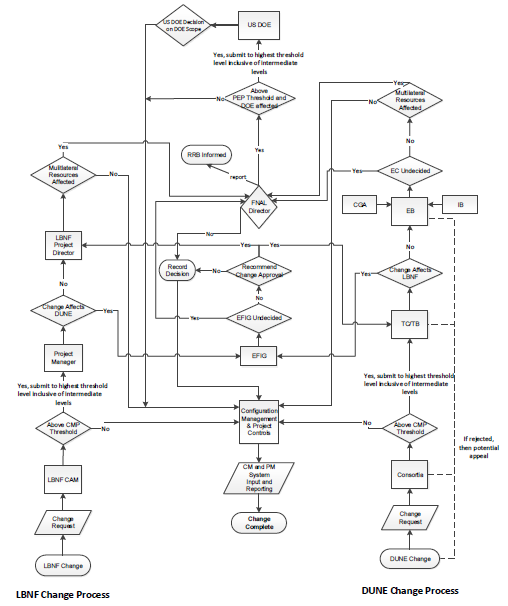
\includegraphics[width=0.95\textwidth]{LBNF-DUNE_ChangeControl_4-1}
\end{dunefigure}


When shop or site work must be performed before the associated %affected 
design
document can be formally revised and re-issued, such changes are
accomplished through the development, approval, and distribution of an
\dword{ecr}. This applies to %process is for 
designs that are
under configuration management. Interdisciplinary reviews are
performed when the \dword{ecr} subject matter may impact other
subsystems. The \dword{ecr} requestor  indicates whether it is a one-time
change or if the change is to be incorporated into the design
documents. Refer to Section~\ref{sec:fdsp-change} for more information on this
process.  This design change control process is applicable to design
changes that may occur during fabrication and for which the change must be
expedited to avoid schedule delays. These types of changes do not
affect technical scope, cost, or schedule. For changes that affect these aspects, 
%technical scope, cost or schedule 
the change control process is defined in
Sections~\ref{sec:dune_changecontrol} and~\ref{sec:tc_change control}.

\section{Design}

The \dword{dune} design process provides appropriate control of design
inputs and design products. The primary design inputs are the
\dword{dune} scientific and engineering requirements (e.g., physics
requirements, detector requirements, specifications, drawings,
engineering reports) as discussed in
Section~\ref{sec:fdsp-coord-requirements}.

The basis of the design process requires sound engineering judgment
and practices, adherence to scientific principles, and use of
applicable orders, codes, and standards. This basis of the design
process naturally incorporates environment, health, and safety
concerns.

\subsection{Design Process}

The \dword{lbnf-dune} Systems Engineering website
documentation defines the scope of design work for any given
scientific/engineering work group. From this source, work groups
will begin preliminary design of \dword{dune} by breaking their work
down into sets of engineering drawings, specifications and
reports. This is the design output.

Throughout the design process, engineers and designers work with
consortium leaders and the \dword{lbnf-dune} \dword{qa} manager to
determine \dword{qa} inspection criteria of fabricated products and
installations. Close coordination must be made with \dword{dune}
scientists to assure the engineering satisfies the scientific
requirements of the experiment. Configuration management as documented
in the \dword{lbnf-dune} \dword{cmp} will be
systematically implemented for \dword{dune}. Final Design work sets
the final \dword{qa} parameters for the parts, assemblies and
installations. Design during final design and production is confined
to change-controlled changes, as above, and to minor changes necessary
to facilitate production, drawing error correction, material
substitutions and similar functional areas.

\subsection{Design Verification and Validation}
\label{sec:verification}

Design is verified and validated to an extent commensurate with its
importance to safety, complexity of design, degree of standardization,
state of the art, and similarity to proven design
approaches. Acceptable verification methods include but are not
limited to any one or a combination of (1) design reviews, (2)
alternative calculations, and (3) prototype, qualification testing,
and/or (4) comparison of the new design with a similar proven design
if available. Verification work must be completed before approval and
implementation of the design.

Design reviews will verify and validate that the following criteria
are met at the appropriate milestone:
\begin{itemize}
 \item adherence to requirements,
 \item technical adequacy of the design,
 \item adequacy of work instructions,
 \item thoroughness of specifications,
 \item test results,
 \item adequacy of technical reports,
 \item adequacy of design calculations and drawings,
 \item reliability and maintainability, and
 \item calibration program for measurement and test equipment.
\end{itemize}
The \dword{dune} Review Plan as discussed in
Chapter~\ref{vl:tc-review} describes the design reviews recommended
for %its 
particular consortia.

Wherever the design method involves the use of
computer software to make engineering calculations or static dynamic
models of the structure, system, or a component's functionality, the
software must be verified to demonstrate that the software produces
valid results. The verification must be documented in a formal
report of validation that is maintained in records that are accessible
for inspection. However, exemptions may be made for commercially
available software that is widely used and for codes with an extensive
history of refinement and use by multiple institutions. Exemptions
affecting systems or components will be identified to the
\dword{lbnf-dune} Systems Engineering team.

Critical software and firmware computer codes, especially those codes
that are involved in controlling \dword{dune} \dword{daq}, are also subject to reviews for verification and
validation. Some items to be considered during computer code review
are
\begin{itemize}
\item adequacy of code testing scheme,
\item code release control and configuration management,
  \item output data verification against code configuration,
  \item verification that code meets applicable standards, 
  \item verification of code compatibility to other systems that use
    the data,
  \item verification that code meets applicable hardware requirements,
  \item adequacy of code maintenance plans, and
  \item adequacy of code and data backup systems.
\end{itemize}

Validation ensures that any given design product conforms to \dword{dune}
requirements.
During reviews, validation of conformity to requirements
follows verification that the engineering design or computer code
meets all criteria. Engineering designs and computer codes are
validated, preferably before procurement, manufacture, or
construction; but no later than acceptance and use of the item; this
is to ensure the design or computer code
\begin{itemize}
 \item meets \dword{dune} requirements,
 \item contains or makes reference to acceptance criteria, and
 \item identifies all characteristics crucial to the safe and proper
   use of the equipment or system and its associated interfaces.
\end{itemize}

Each inspection, test, or review will feed the \dword{qa} evaluation
process, which is a comparison of results with acceptance criteria, to
determine acceptance or rejection. Rejection identifies the need for
Quality Improvement based on Section~\ref{sec:quality_improvement}. In
some cases, the outcome of the Quality Improvement process may be to
request one or more changes to the design requirements.

\dword{qa} reporting formality escalates as the significance of the
inspection, test or review nonconformance increases. Higher levels of
management must be aware of and participate in the correction of the
most significant nonconformance. Section~\ref{sec:quality_improvement}
identifies the required course of action when nonconformance is
encountered.

\section{Procurement}

\subsection{Procurement Controls}

Procurement controls will be implemented to ensure that
purchased items and services meet \dword{dune} requirements and comply
with the \dword{lbnf-dune} \dword{qa} plan.  The consortium members
requesting procurement of items and services are responsible for
providing all documentation that adequately describes the item or
service being procured so that the supplier can understand the 
requirements for consortium acceptance. Development of this documentation
may be achieved through the involvement of consortium leaders and
established review and approval systems. The following factors will be
considered for review and approval of this documentation:
\begin{itemize}
 \item inclusion of technical performance requirements
 \item identification of required codes and standards, laws and
   regulations;
 \item inclusion of acceptance criteria, including requirements for
   receiving inspection and/or source inspection;
 \item \dword{dune} requirements for vendor qualifications and
   certifications;
 \item \dword{dune} intention to perform acceptance sampling in lieu
   of full inspection and test item acceptance.
\end{itemize}
NOTE: For vendor qualification and acceptance of purchased items or
material by consortium members this may be performed under their own
institution requirements.

Previously accepted suppliers will be monitored to ensure that they
continue supplying acceptable items and services. Source surveillance
is the recommended method to ensure that items are free of damage and
that specified requirements are met. Supplier deliveries will be
verified against previously established acceptance criteria.

Unacceptable supplier items or services will be documented. Records
of supplier performance, Inspection Test Records (ITR), and
contract-required submittals, are kept for future procurement
consideration.

Inspections will be conducted to detect counterfeit and/or suspect
parts. For work funded by \dword{doe}, when counterfeit or suspect parts
are found, they will be identified, segregated, and disposed of in
accordance with the \fnal Quality Assurance Manual Chapter 12020
Suspect/Counterfeit Items (S/CI) Program. \dword{dune} consortia may
use their own institutional procedure for counterfeit/suspect parts.

\subsection{Inspection and Acceptance Testing}

Inspection and testing of electrical, mechanical, and structural
components, and associated services and processes by consortium members
will be conducted using acceptance and performance criteria. ITR
forms, travelers, and a traveler database are the primary tools used
to organize this activity. Inspections will be conducted in accordance
with the graded approach.

Once equipment is received at \dword{sdwf}, the equipment is 
inspected for shipping damage and accuracy against the bill of lading. 
Consortium members perform any additional inspection and testing that 
is required by their design documents either at \dword{sdwf} or 
underground in the clean room as the equipment is prepared for 
installation.

Equipment used for all inspections and tests will be calibrated and
maintained. Calibration will be controlled by a system or systems
making appropriate use of qualified calibration service
providers. Consortium leaders must ensure that equipment requiring
calibration have their calibration status identified on the item or
container, are traceable back to the calibration documentation, and are
tracked to ensure the equipment is calibrated at the required
interval. The \dword{lbnf-dune} \dword{qa} manager 
oversees and supports the \dword{dune} calibration programs.

\section{Assessments}

\subsection{Management Assessments}

Management assessments may be performed by the consortia or \dword{tc}
to evaluate their own management processes (self-assessment) and their
implementation in order to identify noteworthy practices, uncover issues,
identify corrective actions, verify meeting of deliverables, and
ensure that work being performed is satisfactory and done according to the 
requirements. The performance of management assessments is a critical
assurance activity.

\dword{dune} \dword{tc} will monitor progress
of objectives and goals in the consortia to assess whether work is
performed and resources are allocated to meet those objectives and
goals. \dword{dune} \dword{tc}  is responsible for monitoring the
resolution of items identified from assessments, assigning
responsibility for resolution, identifying appropriate timeframes for
resolution, ensuring actions are finalized with appropriate objective
evidence, and documented.

The \dword{lbnf-dune} \dword{qa} manager monitors adequacy of
assessments and progress of corrective actions, and sponsors or conducts
periodic assessments of the effectiveness of implementation of the \dword{qa}
program throughout the \dword{dune} project.




\subsection{Independent Assessments}

The \dword{lbnf-dune} \dword{qa} manager will plan reviews as
independent assessments to assist the \dword{dune} \dword{tcoord} in
identifying opportunities for quality or performance-based improvement,
and to ensure compliance with specified requirements. Independent
assessments of the \dword{dune} projects can be requested by
\dword{dune} management. Independent assessments typically focus on
quality or \dword{esh} management systems, self-assessment programs, or
other organizational functions identified by management. The
\dword{dune} project uses a formal process for assigning
responsibility in response to recommendations from independent
assessments. These recommendations are tracked to closure.

%%%
Personnel conducting independent assessments must be technically
qualified and knowledgeable in the areas assessed. A qualified lead
assessor (auditor), who is a Subject Matter Expert (SME) in the
technical area of assessment, is required. The team may include other
SMEs to evaluate the adequacy and effectiveness of activities only if
they are not responsible for the work being assessed.

The \fnal directorate appoints an independent Long Baseline Neutrino
Committee (LBNC) to advise it and \dword{dune} Management. The role of
this standing committee is described in the \dword{lbnf-dune}
project management plan (PMP). The \dword{doe} and other funding agencies perform external
assessments that provide an objective view of performance and thus
contribute to the independent assessment process. Since such
assessments are not under the control of \dword{dune}, they are not
necessarily considered a part of the independent assessment
criterion. However, \dword{dune} management considers external
assessment results when determining the scope and schedule of
independent assessments.

\section{\dshort{dune} Quality Control}
  
The \dword{dune} consortia are a geographically diverse group of institutions,
collaborating across three continents to fabricate a single integrated
system. As such, careful planning and control of component
fabrication, assembly and testing must be maintained. Each of the
major system components will be fabricated in accordance with
documented procedures and drawings.  These procedures will detail the
inspection and test requirements for each component to ensure that they
meet the requisite specifications prior shipment to \dword{surf}.
Each consortium is responsible for developing the procedures, \dword{qc}
plans, and test plans.

Required inspections and tests during fabrication and installation are
defined in the consortium \dword{tdr} sections. These inspections and tests may
be performed from receipt of material, during fabrication and final
acceptance. For critical equipment source inspection may be performed
in addition. The inspections and tests will be documented on \dword{qc} plans,
travelers, test reports, as applicable.  The procedures will define
the documentation method.

All data from the fabrication and \dword{qc} processes will be maintained in a
database that allows the information to be accessed %if needed
during installation. Each consortium will define the requirements for
the information to be stored in the database. The consortium \dword{tdr}
sections contain information on how they are utilizing the database.

In the case of a nonconformance, the nonconformance will be documented
by the fabrication facility and a recommended disposition will be
provided and forwarded to the consortium technical lead.  If the
disposition is to scrap or rework so that the item meets the requirements
of the specification, the notification to the consortium lead will be %%
for information only, and work can continue on performing the
disposition.  If the disposition is ``use as is'' or ``repair'' (where the
item is repaired to meet the functionality but remains in
noncompliance with the specification requirements), work on the item
stops until the disposition has been approved by the design
authority, the consortium technical lead and the \dword{tcoord}.  The \dword{tcoord}
approves the disposition to ensure it does not affect any
other \dword{dune} components during integration. The item will be
re-inspected or tested after completion of the disposition to ensure
that it meets the requirements.

\subsection{\dshort{apa} Quality Control}

Flatness of the \dword{apa} support frame is a key feature and is
defined as the minimum distance between the two parallel planes that 
contain all the points on the surface of the \dword{apa}. After
assembly of the \dword{apa} frame, a laser survey is performed on
the bare frames before  delivery to an \dword{apa}
production site. Three sets of data are compiled into a map that shows
the amount of bow, twist, and fold in the frame. A visual file is also
created for each \dword{apa} from measured data. During \dword{apa}
wiring at the production sites, a final frame survey is completed
after installation of all electrical components, and the as-built
plane-to-plane separations are measured to verify that the
distance between adjacent wire planes meets the tolerances.

Another check performed at the \dword{apa} production site before the
frame is transferred to a winder is necessary to confirm sufficient
electrical contact between the mesh sub-panels and the \dword{apa}
support frame. A resistance measurement is taken immediately after
mesh panel installation for all 20 panels before wiring begins.

All components require inspection and \dword{qc} checks before use on an
\dword{apa}. Most of these tests will be performed at locations other than the
\dword{apa} production sites by institutions within the consortium before the
hardware is shipped for use in \dword{apa} construction. This distributed
model for component production and \dword{qc} is key to enabling the efficient
assembly of \dword{apa}s at the production sites. The critical path components
are the support frames (one per \dword{apa}), grounding mesh panels (20 per
\dword{apa}), and wire carrier boards (204 per \dword{apa}).

The tension of every wire will be measured during production to ensure
that wires have a low probability of breaking or moving excessively in the
detector. Every channel on the completed \dwords{apa} will also be tested for
continuity across the \dword{apa} and isolation from other channels.

A cold testing facility sized for DUNE \dword{apa}s exists at the 
Physical Sciences Laboratory (PSL) at the University of Wisconsin
 that can be
used for such tests. Throughout the construction project, it is
anticipated that 10\% of the produced \dwords{apa} will be shipped to PSL for
cold cycling. This amounts to about one \dword{apa} per year per production site
during the project. %It is planned that 
All \dwords{apa} will still be cold
tested during integration at \dword{surf} and before installation in the \dword{spmod}. % DUNE cryostats. 
All active detector components are shipped to the \dword{sdwf} 
before final transport to \dword{surf}. During the storage period, the wire
tensions are measured on all \dwords{apa} to ensure that the transport has
not damaged the wires.

After unpacking an \dword{apa}, a visual inspection is performed, and
wire continuity and tension are measured again. Definite
guidance for the acceptable tension values will be available to inform
decisions on the quality of the \dword{apa}. Clear pass/fail criteria will be
provided as well as clear procedures to deal with individual wires
lying outside the acceptable values. In addition, a continuity test
and a leakage current test is performed on all channels and the data
recorded in the database.

\subsection{\dshort{hv} Quality Control}

The \dword{hv} consortium has developed a comprehensive \dword{qc}
plan for the production, shipping, and installation of the
\dword{spmod} \dword{hv} components. Inventory tagging and tracking
each component is crucial. Documentation in the form of printed
checklists is maintained. Travelers will have been replaced by a system
of tags (``cattle tags'') attached to the units with bar codes that are associated with 
%key to 
electronic
\dword{qc} data. \fixme{check}

Power supplies used in a \dword{spmod} are tested before
installation. Output voltages and currents must be checked on a known
load. The feedthrough and filters are tested at the same time,
with the planned power supply. The feedthrough must be verified to
hold the required voltage in \dword{tpc}-quality \dword{lar} for several days.

The \dword{qc} tests of the \dwords{hvdb} %Voltage Divider Boards 
require that all
individual resistors and varistors are submitted to a warm and cold
(87 K) current-voltage measurement. This forms the basis for selecting
components that meet specifications; all electrical components must
pass visual inspection for mechanical damage and all measurement values
(resistance, clamping voltage) must be within 2$\sigma$ of the mean for the
entire sample both in warm and cold tests.

The \dword{qc} process for mechanical components starts at the production
factories by attaching a cattle tag with a unique code to each
production element. A file linked to each code contains the individual
measurements and properties contained in the \dword{qc} checklists for that
element.

\subsection{\dshort{tpc} Electronics Quality Control}

All \dwords{asic} will be tested in \dword{ln} before they are mounted
on the \dwords{femb}; cryogenic testing of the \dwords{femb} is also
planned.  Capacitors and resistors will be
cryogenically tested on a sample basis of a few components from each
reel. Some other components installed on the \dwords{femb}, e.g., 
voltage regulators and crystals, will be qualified in \dword{ln}
before being mounted on the \dwords{femb}.

The \dwords{pcb} for the \dwords{femb} will be tested by the
vendor for electrical continuity and shorts. A visual inspection of
the boards is then performed before installing the discrete components
and the \dwords{asic}. This inspection is repeated after
installation and before the functionality test, which for \dword{dune}
will be performed in \dword{ln}.  After assembly, each \dword{femb}
is tested in \dword{ln} using the current \dword{cts}.

Checks will be performed on all cables during production at room
temperature, before installation and connection to the
\dwords{femb}. These tests  involve continuity and resistance
measurements on the low voltage power and the bias voltage cables, and
bit-error rate measurements on the clock/control and data readout
cables. Connectors will be visually inspected to ensure that they show
no sign of damage. Further tests will take place when the \dword{apa}s
are tested in the \coldbox{}es at \dword{surf} prior to installation
inside the cryostat.

On each cryostat penetration there are two flanges for the \dword{ce}
and one for the \dword{pd} system. The crossing tubes with their spool
pieces are fabricated by industry and tested by vendors to be leak and
pressure proof. The flanges are assembled at consortium institutions
responsible for the \dword{tpc} electronics and \dword{pd} system; the
flanges must undergo both electrical and mechanical tests to ensure
their functionality. Electrical tests comprise checking all the
signals and voltages to ensure they are passed properly between the
two sides of the flange and that no shorts exist. Mechanical tests
involve checking that the flange itself is leak and pressure proof.

\subsection{\dshort{pd} Quality Control}

Materials certification is required (in the \dword{fnal} materials test
stand and other facilities) to ensure materials' compliance with
cleanliness requirements. Cryogenic testing of all materials to be
immersed in \dword{lar} is done to ensure satisfactory performance through repeated
and long-term exposure to \dword{lar}. Special attention will be paid to
cryogenic behavior of fused silica and plastic materials (such as
filter plates and wavelength-shifters), \dwords{sipm}, cables, and
connectors. Testing will be conducted both on small-scale test
assemblies (such as the small test cryostat at Colorado State University (CSU)) and full-scale
prototypes (such as the full-scale CDDF cryostat at CSU). Mechanical
interface testing, beginning with simple mechanical go/no-go gauge
tests, followed by installation into the \dword{pdsp2} system, and
finally full-scale interface testing of the \dword{pd} system into the final
pre-production \dword{tpc} system models will be done; as well as full-system readout tests of the
\dword{pd} readout electronics, including trigger generation and timing,
and tests for electrical interference between the \dword{tpc} and \dword{pd}
signals.

Prior to the start of fabrication, a manufacturing and \dword{qc} plan will be
developed detailing the key manufacturing, inspection, and test
steps. The fabrication, inspection, and testing of the components will
be performed in accordance with documented procedures. This work will
be documented on travelers and applicable test or inspection
reports. Records of the fabrication, inspection and testing will be
maintained. When a component has been identified as being in
noncompliance to the design, the nonconforming condition will be
documented, evaluated and dispositioned as one of (1) use-as-is (does not meet
design but can meet functionality as it is), (2) rework (bring into
compliance with design), (3) repair (will be brought to meet functionality
but will not meet design), or (4) scrap. For products with a disposition
of use-as-is or repair, the nonconformance documentation is
submitted to the design authority for approval. All \dword{qc} data (from
assembly and pre- and post-installation into the \dword{apa}) will be directly
stored to the \dword{dune} database for ready access. % of all \dword{qc} data.

Monthly summaries of key performance metrics (to be defined) will be
generated and inspected to check for quality trends. Based on the
\dword{pdsp} model, we expect to conduct the following production
testing prior to shipping from assembly site. 
\begin{itemize}
\item dimensional checks of
critical components and completed assemblies to ensure that
system interfaces ar satisfactory;
\item  post-assembly cryogenic checkouts of \dword{sipm} mounting
\dwords{pcb} (prior to assembly into \dword{pd} modules);
\item module dimensional
tolerances using go/no- go gauge set; and 
\item warm scan of complete module
using motor-driven \dword{led} scanner (or UV \dword{led} array).  
\end{itemize}
Following shipping
to the USA reception and checkout facility but prior to storage at
\dword{sdwf}, we will conduct mechanical inspection, a warm scan (using identical scanner to
initial scan), and cryogenic testing of completed modules (at the CSU CDDF or
similar facility).

Following delivery to the underground integration cleanroom, prior to and
during integration and Installation, we will 
\begin{itemize}
\item conduct  a warm scan (using identical
scanner to initial scan);
\item  complete visual inspection of module against
a standard set of inspection points, with photographic records kept
for each module;
\item conduct end-to-end cable continuity and short circuit tests
of assembled cables; 
\item perform a \dword{fe} electronics functionality
check  
\item perform installation \dword{qc} \dword{pd} system pre-installation testing, following the model established for \dword{pdsp}.
\end{itemize}


Prior to installation in the \dword{apa}, the \dword{pd} modules will undergo a warm
scan in a scanner identical to the one at the \dword{pd} module assembly
facility and we will compare the results. The module will also 
undergo a complete visual inspection for defects, and a set of
photographs of selected critical optical surfaces will be taken and entered
into the \dword{qc} record database. Following installation into the \dword{apa} and
cabling, an immediate check for electrical continuity to the \dwords{sipm}
will be conducted. Following the mounting of the \dword{tpc} \dword{ce}
and the \dwords{pd}, the entire \dword{apa} will undergo a cold system
test in a gaseous argon \coldbox, similar to that performed for
\dword{pdsp}. During this test and prior to installation, the \dword{pd} system 
will undergo a final
integrated system check, checking dark and
\dword{led}-stimulated \dword{sipm} performance for all channels, checking for
electrical interference with the \dword{ce}, and confirming
compliance with the detector grounding scheme.

\subsection{Calibration Quality Control}

The manufacturer and the institutions in charge of devices will
conduct  series of tests to ensure the equipment can perform its
intended function as part of \dword{qc}. \dword{qc}
also includes post-fabrication tests and tests run after shipping and
installation. The overall strategy for the calibration devices is to
test the systems for correct and safe operation first in dedicated test
stands, then at \dword{pdsp2}, then as appropriate near \dword{surf},
and finally underground. Electronics and racks associated with each full
system will be tested before transporting them underground. Each calibration
system undergoes specific tests.
\begin{itemize}
\item Ionization Laser System: For assembly and operation of the laser
  and feedthrough interface, %this will be 
  the test is carried out on a mock-up
  flange for each of the full hardware sets (periscope, feedthrough,
  laser, power supply, and electronics). All operational parts (UV
  laser, red alignment laser, trigger photodiode, attenuator,
  diaphragm, movement motors, and encoders) are tested for
  functionality before being transported underground.
\item Photoelectron Laser System: The crucial test is to measure the
  light transmission of all fibers at 266 nm. A suitable transmission
  acceptance threshold will be established based on studies during the
  development phase. Studies to estimate the number of photoelectrons
  emitted as a function of intensity (based on distance of fiber
  output to the metallic tab) will also be undertaken.
\item Laser Beam Location System: For the \dword{lbls}, to ensure uniformity
  across all clusters, the main test is to verify 
   that the PIN diodes are all functional and that their light
  detection efficiency is within a specified range. For the mirror-based system, the reflectivity
  of all mirrors will  be tested prior to assembly.
\item Pulsed Neutron Source System: The first test will be safe
  operation of the system in a member institution radiation-safe
  facility. Then the system will be validated at \dword{pdsp2}. The
  same procedure will be carried out for any subsequent devices before
  the devices are transported to \dword{surf} and underground. System
  operation will be tested with shielding assembled to confirm safe
  operating conditions and sufficient neutron yields using an external
  dosimeter as well as with the installed neutron monitor.
\end{itemize}

\subsection{\dshort{daq} Quality Control}

SP-DAQ-6 Data verification: The \dword{daq} must check integrity of data at
every data transfer step. It only deletes data from the local
storage after confirmation that data have been correctly recorded to
permanent storage. Data integrity checking is fundamental to ensure
data quality. The high overall experiment uptime goal requires that the \dword{daq} 
be stringently designed for reliability, fault tolerance, and
redundancy  -- criteria that aim to reduce overall downtime. The \dword{daq}
monitors the quality of the detector data and of its own operational
status, performs automated error detection, and has recovery
capabilities.

The \dword{eb} subsystem provides bookkeeping
functionality for the raw data. This  includes the documenting of
simple mappings, such as which trigger is stored in which raw data
file, as well as more sophisticated quality checks. For example, it
will know which time windows and geographic regions of the detector
are requested for each trigger, and in the unlikely event that some
fraction of the requested detector data cannot be stored in the event
record, it will document that mismatch.

Data Quality Monitoring: While the \dword{daqccm} contains an element of
monitoring (Section 7.3.5.4) \fixme{fix}, here \dword{dqm}
refers to a subsystem that quickly analyzes the data in order to
determine the general quality of the detector and \dword{daq} operation. This
 allows operators to promptly detect and respond to any
unexpected changes and assures high exposure times for later physics
analyses.

A \dword{daq} \dword{dqm} will be developed (including
necessary infrastructure, visualization, and algorithms) that 
processes a subset of detector data in order to provide prompt feedback
to the detector operators. This system will be designed to allow it to
evolve as the detector and its data are understood during
commissioning and early operation, and to cope with any evolution of
detector conditions.

While the hardware design will be done at the institutions working in
this area, the production of prototypes and final cards \fixme{cards?} will be
outsourced to companies, allowing for early identification of those
companies that can guarantee a high-quality card production.


\subsection{\dshort{cisc} Quality Control}

The manufacturer and the institution in charge of device assembly will
conduct a series of tests to ensure the equipment can perform its
intended function as part of \dword{qc}. \dword{qc} also includes post fabrication
tests and tests run after shipping and installation. For complex
systems, the entire system will be tested before shipping. Additional
\dword{qc} procedures can be performed underground after installation.

The planned tests for each subsystem are described below.

\subsubsection{Purity Monitors}

The purity monitor system will undergo a series of tests to ensure the
system performs as intended.  These tests %reflect 
are based on the \dword{pdsp}
purity monitor \dword{qc} tests, which included electronic tests with a pulse
generator, mechanical and electrical connectivity tests at cryogenic
temperatures in a cryostat, and vacuum tests for short and full
assemblies in a dewar and in a long vacuum tube.

The \dword{qc} tests for \dword{fd} purity monitors begin with testing
individual purity monitors in vacuum after each is fabricated and
assembled. This test checks the amplitude of the signal generated by
the drift electrons at the cathode and the anode to ensure that the
photocathode can provide sufficient numbers of photoelectrons to
measure the signal attenuation with the required precision, and that
the field gradient resistors all work properly to maintain the drift
field. A smaller version of the assembly with all purity monitors
installed will be tested at the \dword{citf} to ensure the full system
performs as expected in \dword{lar}.

Next, the entire system is assembled on the full-length mounting tubes
to check the connections along the way. Ensuring that all electric and
optical connections are operating properly during this test reduces
the risk of problems once the full system is assembled and ready for
the final test in vacuum. The fully assembled system is placed in the
shipping tube, which serves as a vacuum chamber, and tested at
\dword{surf} before the system is inserted into the cryostat. During
insertion, electrical connections are tested continuously with
multimeters and electrometers.

\subsubsection{Thermometers}

Static T-gradient thermometers: Static T-gradient monitors undergo
three type of tests at the production site before shipment to
\dword{surf}: a mechanical rigidity test, a calibration of all
sensors, and a test of all electrical cables and connectors.

The calibration procedure itself provides \dword{qc} because each set
of sensors goes through five independent measurements. Sensors with
\dword{rms} variation outside the requirement (2 mK for \dword{pdsp}) are
discarded. This calibration also serves as \dword{qc} for the readout
system (similar to the final one) and of the \dword{pcb}-sensor-connector
assembly.

Finally, the cable-connector assemblies are tested; sensors must
measure the expected values with no additional noise introduced by
either cable or connector.

An integrated system test is conducted at a \dword{lar} test facility
at the production site, which has sufficient linear dimension ($>$2 m)
to test a good portion of the system. This ensures that the system
operates in \dword{lar} at the required level of performance. The
laboratory sensor calibration is compared with the in situ calibration
of the dynamic T-gradient monitors by operating both dynamic and
static T-gradient monitors simultaneously.

The last phase of \dword{qc} takes place after installation. The
verticality of each array is checked, and the tensions in the
stainless steel strings adjusted as necessary. Before closing the
flange, the entire readout chain is tested. This allows a test of the
sensor-connector assembly, the cable-connector assemblies at both
ends, and the noise level inside the cryostat. If any sensor presents
a problem, it is replaced. If the problem persists, the cable is
checked and replaced as needed.

\subsubsection{Dynamic T-gradient thermometers}

Before installation, temperature sensors are tested in \dword{ln} to
verify correct operation and to set the baseline calibration for each
sensor with respect to the absolutely calibrated reference sensor.

Warm and cold temperature readings are taken with each sensor after it
is mounted on the \dword{pcb} board and the readout cables are soldered.  The
sensor readout is taken for all sensors after the cold cables are
connected to electric feedthroughs on the flange and the warm cables
outside of the cryostat are connected to the temperature readout
system.

The fully assembled rod is connected to the pinion and gear, and moved
with the stepper motor on a high platform many times to verify
repeatability, possible offsets, and any uncertainty in the
positioning. Finally, repeating this test so many times will verify
the sturdiness of the system.

The full system is tested after it is installed in the cryostat; both
motion and sensor operation are tested by checking sensor readout and
vertical motion of the system.

To address the quality of individual precision sensors, the same
method as for the static T-gradient monitors is used. The \dword{qc}
of the sensors is part of the laboratory calibration.

After mounting six sensors with their corresponding cables, a SUBD-25
connector is added, and the six sensors are tested at room
temperature. All sensors must give values within specifications.

\subsubsection{Gas Analyzers}

The gas analyzer modules are checked for both zero and the span values
using a gas-mixing instrument and two gas cylinders, one having a zero
level of the gas analyzer contaminant species and the other %cylinder
having a known percentage of the contaminant gas. This verifies the
proper operation of the gas analyzers. When they are installed at
\dword{surf}, this process is repeated prior to commissioning the cryostat. \fixme{the cryostat, not the detector?}

\subsubsection{Liquid Level Monitoring}

The manufacturer will provide the \dword{qc} for the differential pressure
level meters. The capacitive sensors will be tested with a modest
sample of \dword{lar} in the laboratory before  installation. After
installation, they are tested in situ using a suitable dielectric in
contact with the sensor.

\subsubsection{Pressure Meters}

The manufacturer will provide the \dword{qc} for the pressure meters.

The pressure sensors will be tested with a modest sample of gaseous
argon in the laboratory before they are installed. After installation,
they are tested in situ at atmospheric pressure. The whole pressure
readout chain, (including slow controls PLC and WINCC conversion) will
also be tested and cross-checked with \dword{lbnf} pressure sensors.

\subsubsection{Cameras}

Before transport to \dword{surf}, each cryogenic camera unit
(comprising the enclosure, camera, and internal thermal control and
monitoring) is checked for correct operation of all features, for
recovery from 87K non-operating mode, for leakage, and for physical
defects. Lighting systems are similarly checked. Operations tests will
verify correct current draw, image quality, and temperature readback
and control. The movable inspection camera apparatus is inspected for
physical defects and checked for proper mechanical operation before
shipping. A checklist is created for each unit, filed electronically
in the \dword{dune} logbook, and a hard copy is sent with each unit.

Before installation, each fixed cryogenic camera unit is inspected for
physical damage or defects and checked at the \dword{citf} for correct
operation of all features, for recovery from 87K non-operating mode,
and for contamination of the \dword{lar}. Lighting systems are similarly
checked. Operations tests verify correct current draw, image quality,
and temperature readback and control.

After installation and connection of wiring, fixed cameras and
lighting are again checked for operation.  The movable inspection
camera apparatus is inspected for physical defects and, after
integration with a camera unit, tested in the facility for proper
mechanical and electronic operation and cleanliness before being
installed or stored. A checklist is completed for each \dword{qc} check
and filed electronically in the \dword{dune} logbook.

\subsubsection{\dshort{led} System}

The entire \dword{led} system is checked before installation to ensure
functionality of light emission. Initial testing of the system begins
with measuring the current when low voltage (1~V) is applied, to check
that the resistive \dword{led} failover path is correct. Next, the
forward voltage is measured using nominal forward current to check
that it is within 10\% of the nominal forward voltage drop of the
\dword{led}, that all of the \dwords{led} are illuminated, and that
each \dword{led} is visible over the nominal angular range. If the
\dwords{led} are infrared, a video camera with the IR filter removed
is used for a visual check.


This procedure is then duplicated with the current reversed for
\dwords{led} oriented in the opposite direction. Initial tests are
performed at room temperature and then repeated in \dword{ln}. Color
shifts in the \dwords{led} are expected and will be noted. A checklist
is completed for each \dword{qc} check and filed electronically in the
DUNE logbook.

Room temperature tests are repeated during and immediately after
installation to ensure that the system has not been damaged during
transportation or installation. Functionality checks of the
\dwords{led} are repeated after the cameras are installed in the
cryostat.

Slow Controls Hardware Networking and computing systems will be
purchased commercially, requiring \dword{qa}. \fixme{qc?}However, the new servers
are tested after delivery to confirm they suffered no damage during
shipping. The new system is allowed to burn in overnight or for a few
days, running a diagnostics suite on a loop in order to validate the
manufacturer’s \dword{qa} process.


\section{ProtoDUNE to DUNE QA Approach}

The approach to \dfirst{qa}/\dfirst{qc} for \dword{dune} is going to be
very similar to the activities and oversight that was performed for
\dword{protodune}.  For \dword{protodune}, the major
\dword{qa}/\dword{qc} activities included review of the consortium
\dword{tdr} \dword{qa}/\dword{qc} sections; assisting the consortia in
development and review of \dword{qc} plans (production and
installation), fabrication, inspection and test procedures,
installation plans and documentation; and the performance of
\dwords{prr} at eleven consortium fabrication facilities.  There was
also \dword{qa} participation in the \dword{protodune} design reviews.
The \dwords{prr} looked at the following criteria:
\begin{itemize}
  \item final \dword{qa} plans for institutions not adopting the
    \dword{lbnf-dune} \dword{qa} Plan;
  \item final production drawings, specifications, and manufacturing
    and test procedures;
  \item final safety documents (i.e., hazard analysis documentation);
  \item component \dword{qc} plan (i.e., travelers, test reports,
    software verification and validation documents, supplier
    documentation);
  \item final procurement documents per institution practice; and
  \item completion and evaluation of prototypes, and review of production
    process and \dword{qc} results.
\end{itemize}
The reviews ensured the facilities
were prepared for production and that any kinks in the processes had been
identified and mitigations performed. %have taken place. 
The positive outcome of
these reviews was the amount of equipment received at \dword{cern} with little
to no damage.

\dwords{ppr} will be performed at the fabrication facilities for the
\dword{dune} detector components. This type of review has been added due to the
larger number of components required and the increased number of
fabrication facilities. The goal of these reviews is to ensure
consistent fabrication processes between the facilities. If an issue
is identified at one facility, it can be communicated to %the other applicable facilities 
others to prevent recurrence. %the same issue occurring.

For \dword{protodune}, installation was performed at \dword{cern} under the
guidance of \dword{cern} policies and procedures. Installation of the
\dword{dune} \dwords{detmodule} at \dword{surf} will fall under similar procedures in the
\dword{lbnf-dune} \dword{qa} plan.
